\documentclass[12pt,a4paper]{article}
\usepackage[utf8]{inputenc}
\usepackage[T2A]{fontenc}
\usepackage[russian, english]{babel}
\usepackage{graphicx}
\usepackage{listings}
\begin{document}
\section{Постановка задачи}
Цели лабораторной работы:
\begin{enumerate}
    \item Язык SQL. Объединения. UNION.
    \item Язык SQL. Соединения. JOIN.
\end{enumerate}
\section{Подготовка тестовых данных}

\begin{lstlisting}[language=SQL]
CREATE TABLE `db_access`.`test_join_1` (
`id` INT NOT NULL,
PRIMARY KEY (`id`));
\end{lstlisting}

\begin{lstlisting}[language=SQL]
CREATE TABLE `db_access`.`test_join_2` (
`id` INT NOT NULL,
PRIMARY KEY (`id`));
\end{lstlisting}

\begin{lstlisting}[language=SQL]
INSERT INTO test_join_1 VALUES (1, 2, 3, 4);
INSERT INTO test_join_2 VALUES (3, 4, 5, 6);
\end{lstlisting}

\begin{lstlisting}[language=SQL]
SELECT id FROM test_join_1;
\end{lstlisting}
\begin{lstlisting}[basicstyle = \tiny\ttfamily, columns = fixed]
+----+
| id |
+----+
|  1 |
|  2 |
|  3 |
|  4 |
+----+
4 rows in set (0.00 sec)
\end{lstlisting}

\begin{lstlisting}[language=SQL]
SELECT id FROM test_join_2;
\end{lstlisting}
\begin{lstlisting}[basicstyle = \tiny\ttfamily, columns = fixed]
+----+
| id |
+----+
|  3 |
|  4 |
|  5 |
|  6 |
+----+
4 rows in set (0.00 sec)
\end{lstlisting}

\section{Объединения}
\begin{lstlisting}[language=SQL]
( SELECT id FROM test_join_1 )
UNION DISTINCT
( SELECT id FROM test_join_2 )
\end{lstlisting}

\begin{lstlisting}[basicstyle = \tiny\ttfamily, columns = fixed]
+----+
| id |
+----+
|  1 |
|  2 |
|  3 |
|  4 |
|  5 |
|  6 |
+----+
6 rows in set (0.00 sec)
\end{lstlisting}

\begin{lstlisting}[language=SQL]
( SELECT id FROM test_join_1 )
UNION ALL
( SELECT id FROM test_join_2 )
\end{lstlisting}

\begin{lstlisting}[basicstyle = \tiny\ttfamily, columns = fixed]
+----+
| id |
+----+
|  1 |
|  2 |
|  3 |
|  4 |
|  3 |
|  4 |
|  5 |
|  6 |
+----+
8 rows in set (0.00 sec)
\end{lstlisting}

\section{Соединения}
\begin{figure}[ht]
    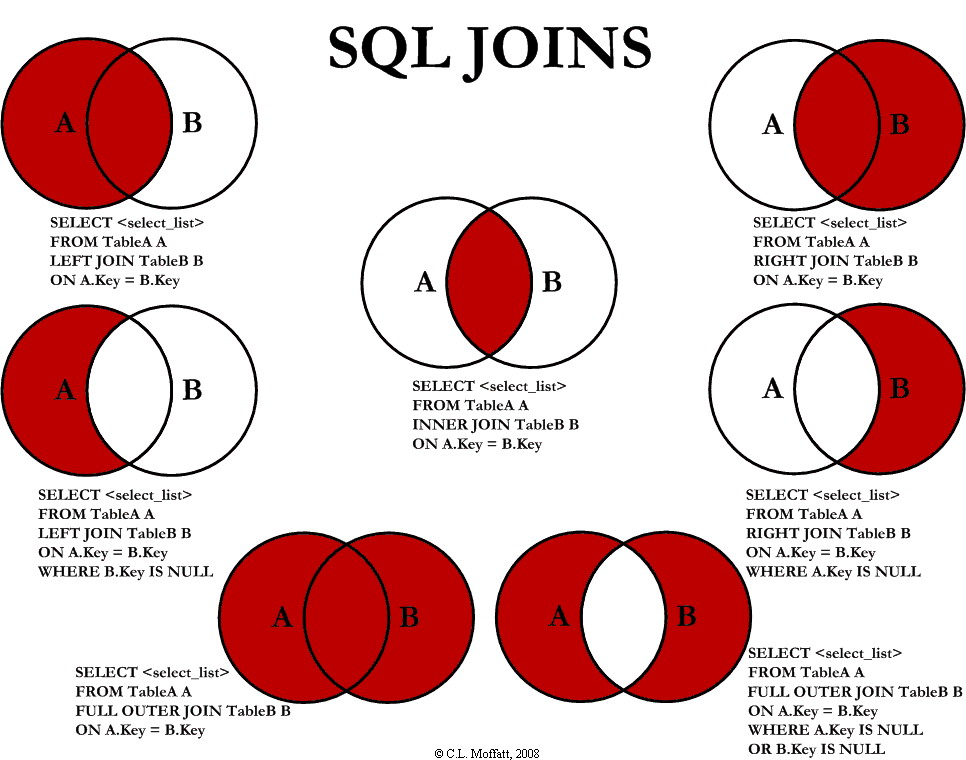
\includegraphics[width=\linewidth]{images/Lab5/joins.jpg}
    \caption{Joins}
    \label{fig:Joins}
\end{figure}
\subsection{CROSS JOIN}

\begin{lstlisting}[language=SQL]
SELECT * FROM test_join_1, test_join_2;
\end{lstlisting}

\begin{lstlisting}[language=SQL]
SELECT * FROM test_join_1 JOIN test_join_2;
\end{lstlisting}

\begin{lstlisting}[language=SQL]
SELECT * FROM test_join_1 CROSS JOIN test_join_2;
\end{lstlisting}

\begin{lstlisting}[basicstyle = \tiny\ttfamily, columns = fixed]
+----+----+
| id | id |
+----+----+
|  1 |  3 |
|  2 |  3 |
|  3 |  3 |
|  4 |  3 |
|  1 |  4 |
|  2 |  4 |
|  3 |  4 |
|  4 |  4 |
|  1 |  5 |
|  2 |  5 |
|  3 |  5 |
|  4 |  5 |
|  1 |  6 |
|  2 |  6 |
|  3 |  6 |
|  4 |  6 |
+----+----+
16 rows in set (0.00 sec)
\end{lstlisting}

\subsection{INNER JOIN}

\begin{figure}[!ht]
    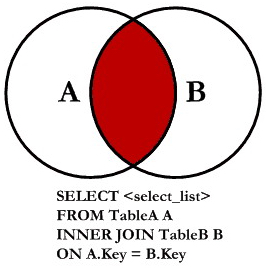
\includegraphics[width=5cm,height=5cm]{images/Lab5/inner_join.jpg}
    \caption{Inner Join}
    \label{fig:InnerJoin}
\end{figure}

\begin{lstlisting}[language=SQL]
SELECT * FROM test_join_1 
INNER JOIN test_join_2 ON test_join_1.id = test_join_2.id;
\end{lstlisting}

\begin{lstlisting}[basicstyle = \tiny\ttfamily, columns = fixed]
+----+----+
| id | id |
+----+----+
|  3 |  3 |
|  4 |  4 |
+----+----+
2 rows in set (0.00 sec)
\end{lstlisting}

\begin{lstlisting}[language=SQL]
SELECT * FROM test_join_1 
INNER JOIN test_join_2 USING (id);
\end{lstlisting}

\begin{lstlisting}[basicstyle = \tiny\ttfamily, columns = fixed]
+----+
| id |
+----+
|  3 |
|  4 |
+----+
2 rows in set (0.00 sec)
\end{lstlisting}

\subsection{LEFT JOIN}
\begin{figure}[!ht]
    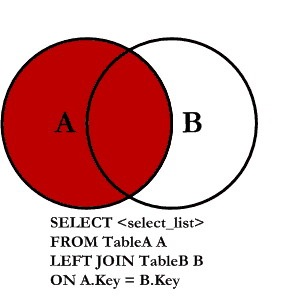
\includegraphics[width=5cm,height=5cm]{images/Lab5/left_join.jpg}
    \caption{Left Join}
    \label{fig:LeftJoin}
\end{figure}
\begin{lstlisting}[language=SQL]
SELECT * FROM test_join_1 LEFT JOIN test_join_2 
ON test_join_1.id = test_join_2.id;
\end{lstlisting}

\begin{lstlisting}[language=SQL]
SELECT * FROM test_join_1 LEFT OUTER JOIN test_join_2 
ON test_join_1.id = test_join_2.id;
\end{lstlisting}

\begin{lstlisting}[basicstyle = \tiny\ttfamily, columns = fixed]
+----+------+
| id | id   |
+----+------+
|  1 | NULL |
|  2 | NULL |
|  3 |    3 |
|  4 |    4 |
+----+------+
4 rows in set (0.00 sec)
\end{lstlisting}

Пример записи через подзапрос.
\begin{lstlisting}[language=SQL]
(
    SELECT test_join_1.id as left_table_id, test_join_2.id FROM test_join_1
	INNER JOIN test_join_2 ON test_join_1.id = test_join_2.id
)
UNION
(
	SELECT test_join_1.id as left_table_id, NULL FROM test_join_1
    WHERE NOT EXISTS(SELECT 1 FROM test_join_2 WHERE test_join_2.id = test_join_1.id)
)
ORDER BY left_table_id
\end{lstlisting}

\begin{figure}[!ht]
    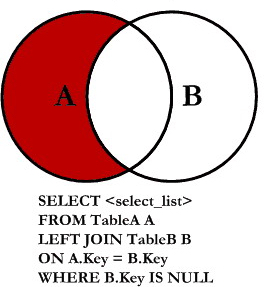
\includegraphics[width=5cm,height=5cm]{images/Lab5/left_join_key.jpg}
    \caption{Left Join Key}
    \label{fig:LeftJoinKey}
\end{figure}

\begin{lstlisting}[language=SQL]
SELECT * FROM test_join_1 LEFT OUTER JOIN test_join_2 
ON test_join_1.id = test_join_2.id
WHERE test_join_2.id IS NULL
\end{lstlisting}

\begin{lstlisting}[basicstyle = \tiny\ttfamily, columns = fixed]
    +----+------+
| id | id   |
+----+------+
|  1 | NULL |
|  2 | NULL |
+----+------+
2 rows in set (0.00 sec)
\end{lstlisting}

Пример записи через подзапрос:

\begin{lstlisting}[language=SQL]
SELECT id FROM test_join_1
WHERE NOT EXISTS (SELECT 1 FROM test_join_2 WHERE test_join_1.id = test_join_2.id)
\end{lstlisting}

\subsection{RIGHT JOIN}

\begin{figure}[!ht]
    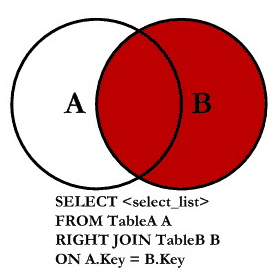
\includegraphics[width=5cm,height=5cm]{images/Lab5/right_join.jpg}
    \caption{Right Join}
    \label{fig:RightJoin}
\end{figure}

\begin{lstlisting}[language=SQL]
SELECT * FROM test_join_1 RIGHT JOIN test_join_2 
ON test_join_1.id = test_join_2.id;
\end{lstlisting}

\begin{lstlisting}[language=SQL]
SELECT * FROM test_join_1 RIGHT OUTER JOIN test_join_2 
ON test_join_1.id = test_join_2.id;
\end{lstlisting}

\begin{lstlisting}[basicstyle = \tiny\ttfamily, columns = fixed]
+------+----+
| id   | id |
+------+----+
|    3 |  3 |
|    4 |  4 |
| NULL |  5 |
| NULL |  6 |
+------+----+
4 rows in set (0.00 sec)
\end{lstlisting}

Пример записи через подзапрос:

\begin{lstlisting}[language=SQL]
(
    SELECT test_join_1.id, test_join_2.id as right_table_id FROM test_join_1
	INNER JOIN test_join_2 ON test_join_1.id = test_join_2.id
)
UNION
(
	SELECT NULL, test_join_2.id as right_table_id FROM test_join_2
    WHERE NOT EXISTS(SELECT 1 FROM test_join_1 WHERE test_join_2.id = test_join_1.id)
)
ORDER BY right_table_id
\end{lstlisting}

\begin{figure}[!ht]
    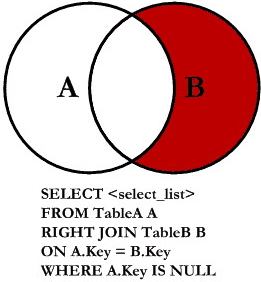
\includegraphics[width=5cm,height=5cm]{images/Lab5/right_join_key.jpg}
    \caption{Right Join Key}
    \label{fig:RightJoinKey}
\end{figure}

\begin{lstlisting}[language=SQL]
SELECT * FROM test_join_1 RIGHT JOIN test_join_2 
ON test_join_1.id = test_join_2.id
WHERE test_join_1.id IS NULL;
\end{lstlisting}

\begin{lstlisting}[basicstyle = \tiny\ttfamily, columns = fixed]
+------+----+
| id   | id |
+------+----+
| NULL |  5 |
| NULL |  6 |
+------+----+
2 rows in set (0.00 sec)
\end{lstlisting}


Пример записи через подзапрос:
\begin{lstlisting}[language=SQL]
SELECT id FROM test_join_2
WHERE NOT EXISTS (SELECT 1 FROM test_join_1 WHERE test_join_2.id = test_join_1.id)
\end{lstlisting}

\subsection{FULL OUTER JOIN}

\begin{figure}[!ht]
    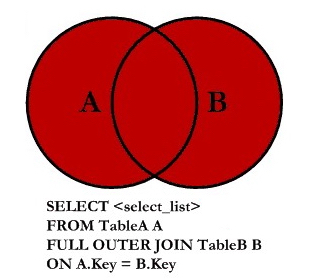
\includegraphics[width=5cm,height=5cm]{images/Lab5/full_outer_join.jpg}
    \caption{Full Outer Join}
    \label{fig:FullOuterJoin}
\end{figure}

\begin{lstlisting}[language=SQL]
(
	SELECT * FROM test_join_1 LEFT JOIN test_join_2 
	ON test_join_1.id = test_join_2.id
)
UNION
(
	SELECT * FROM test_join_1 RIGHT JOIN test_join_2 
	ON test_join_1.id = test_join_2.id
)
\end{lstlisting}

\begin{lstlisting}[basicstyle = \tiny\ttfamily, columns = fixed]
+------+------+
| id   | id   |
+------+------+
|    1 | NULL |
|    2 | NULL |
|    3 |    3 |
|    4 |    4 |
| NULL |    5 |
| NULL |    6 |
+------+------+
6 rows in set (0.00 sec)
\end{lstlisting}

\begin{figure}[!ht]
    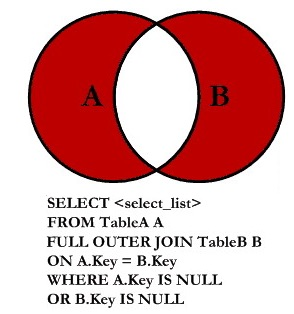
\includegraphics[width=5cm,height=5cm]{images/Lab5/full_outer_join_key.jpg}
    \caption{Full Outer Join Key}
    \label{fig:FullOuterJoinKey}
\end{figure}

\begin{lstlisting}[language=SQL]
(
	SELECT * FROM test_join_1 LEFT JOIN test_join_2 
	ON test_join_1.id = test_join_2.id
    WHERE test_join_2.id IS NULL
)
UNION
(
	SELECT * FROM test_join_1 RIGHT JOIN test_join_2 
	ON test_join_1.id = test_join_2.id
    WHERE test_join_1.id IS NULL
)
\end{lstlisting}

\begin{lstlisting}[basicstyle = \tiny\ttfamily, columns = fixed]
+------+------+
| id   | id   |
+------+------+
|    1 | NULL |
|    2 | NULL |
| NULL |    5 |
| NULL |    6 |
+------+------+
4 rows in set (0.00 sec)
\end{lstlisting}

\subsection{SELF JOIN}
\begin{lstlisting}[language=SQL]
SELECT * FROM test_join_1 FIRST [JOIN TYPE] test_join_1 SECOND
\end{lstlisting}

Пример. Найти пары чисел идущих по возрастанию.

\begin{lstlisting}[language=SQL]
SELECT * FROM test_join_1 FIRST, test_join_1 SECOND
WHERE SECOND.id = FIRST.id+1
\end{lstlisting}
\begin{lstlisting}[basicstyle = \tiny\ttfamily, columns = fixed]
+----+----+
| id | id |
+----+----+
|  1 |  2 |
|  2 |  3 |
|  3 |  4 |
+----+----+
3 rows in set (0.00 sec)
\end{lstlisting}

\section{Примеры запросов}

Получить сумму всех профессий из двух таблиц TitlePrincipalsProfession и NameProfession.

\begin{lstlisting}[language=SQL]
SELECT profession, SUM(count) as professions_summ FROM 
(	
    (SELECT professionID, COUNT(professionID) as count FROM name_profession GROUP BY professionID)
    UNION
    (SELECT professionID, COUNT(professionID) as count FROM title_principals_profession GROUP BY professionID)
) as professions_union
INNER JOIN profession ON professions_union.professionID = profession.professionID
GROUP BY profession
ORDER BY professions_summ DESC
LIMIT 10
\end{lstlisting}

\begin{lstlisting}[basicstyle = \tiny\ttfamily, columns = fixed]
+-------------------+------------------+
| profession        | professions_summ |
+-------------------+------------------+
| actor             |           843352 |
| actress           |           491744 |
| miscellaneous     |           482696 |
| producer          |           323650 |
| writer            |           308877 |
| camera_department |           192286 |
| director          |           190030 |
| art_department    |           181082 |
| visual_effects    |           107347 |
| composer          |            97795 |
+-------------------+------------------+
10 rows in set (1.24 sec)
\end{lstlisting}

Найти фильмы для которых в базе данных нет информации об актерском составе.

\begin{lstlisting}[language=SQL]
SELECT DISTINCT originalTitle, runtimeMinutes, numVotes, averageRating FROM title 
LEFT JOIN title_principals_profession ON title.titleID = title_principals_profession.titleID
INNER JOIN title_rating ON title.titleID = title_rating.titleID
WHERE title_principals_profession.titleID IS NULL AND titleType = 'movie'
ORDER BY numVotes DESC, averageRating DESC
LIMIT 5
\end{lstlisting}

\begin{lstlisting}[basicstyle = \tiny\ttfamily, columns = fixed]
+-------------------------------------------+----------------+----------+---------------+
| originalTitle                             | runtimeMinutes | numVotes | averageRating |
+-------------------------------------------+----------------+----------+---------------+
| Dunkirk                                   |            106 |   483948 |           7.9 |
| Get Out                                   |            104 |   424443 |           7.7 |
| Deadpool 2                                |            119 |   419898 |           7.7 |
| Split                                     |            117 |   377084 |           7.3 |
| Three Billboards Outside Ebbing, Missouri |            115 |   363790 |           8.2 |
+-------------------------------------------+----------------+----------+---------------+
\end{lstlisting}

Найти фильмы актеров киноиндустрии в которых они снимались, но не получили за них известность.

\begin{lstlisting}[language=SQL]
SELECT title_principals_profession.nameID, originalTitle, primaryName, characters FROM name_known_for_title
RIGHT JOIN title_principals_profession ON name_known_for_title.nameID = title_principals_profession.nameID 
AND name_known_for_title.titleID = title_principals_profession.titleID
INNER JOIN profession ON title_principals_profession.professionID = profession.professionID
INNER JOIN title ON title_principals_profession.titleID = title.titleID
INNER JOIN title_rating ON title_principals_profession.titleID = title_rating.titleID
INNER JOIN name ON title_principals_profession.nameID = name.nameId
WHERE name_known_for_title.titleID IS NULL AND profession = 'actor'
ORDER BY title_rating.numVotes DESC, title_rating.averageRating DESC
LIMIT 10
\end{lstlisting}

\begin{lstlisting}[basicstyle = \tiny\ttfamily, columns = fixed]
+-----------+---------------------------------------+---------------------+------------------------------+
| nameID    | originalTitle                         | primaryName         | characters                   |
+-----------+---------------------------------------+---------------------+------------------------------+
| nm0000151 | The Shawshank Redemption              | Morgan Freeman      | ["Ellis Boyd 'Red' Redding"] |
| nm0000093 | Fight Club                            | Brad Pitt           | ["Tyler Durden"]             |
| nm0001570 | Fight Club                            | Edward Norton       | ["The Narrator"]             |
| nm0000237 | Pulp Fiction                          | John Travolta       | ["Vincent Vega"]             |
| nm0322513 | Game of Thrones                       | Iain Glen           | ["Jorah Mormont"]            |
| nm0000198 | The Dark Knight Rises                 | Gary Oldman         | ["Commissioner Gordon"]      |
| nm0000288 | The Dark Knight Rises                 | Christian Bale      | ["Bruce Wayne"]              |
| nm0001557 | The Lord of the Rings: The Two Towers | Viggo Mortensen     | ["Aragorn"]                  |
| nm0089217 | The Lord of the Rings: The Two Towers | Orlando Bloom       | ["Legolas"]                  |
| nm0000190 | Interstellar                          | Matthew McConaughey | ["Cooper"]                   |
+-----------+---------------------------------------+---------------------+------------------------------+
\end{lstlisting}

Получить список фильмов и задействованных членов съемочной группы с одинаковым годом рождения.

\begin{lstlisting}[language=SQL]
SELECT F_Principals.titleID, F.primaryName, F.birthYear, primaryTitle, numVotes, averageRating FROM imdb_db_part.name F
CROSS JOIN imdb_db_part.name S
INNER JOIN title_principals_profession F_Principals ON F.nameID = F_Principals.nameID
INNER JOIN title_principals_profession S_Principals ON S.nameID = S_Principals.nameID
INNER JOIN title_rating ON F_Principals.titleID = title_rating.titleID
INNER JOIN title ON F_Principals.titleID = title.titleID
WHERE F.birthYear = S.birthYear AND F.nameID != S.nameID AND F_Principals.titleID = S_Principals.titleID
ORDER BY numVotes DESC, averageRating DESC, birthYear ASC
LIMIT 20
\end{lstlisting}

\begin{lstlisting}[basicstyle = \tiny\ttfamily, columns = fixed]
+-----------+------------------------+-----------+---------------------------------------------------+----------+---------------+
| titleID   | primaryName            | birthYear | primaryTitle                                      | numVotes | averageRating |
+-----------+------------------------+-----------+---------------------------------------------------+----------+---------------+
| tt0137523 | Cein Chaffin           |      1957 | Fight Club                                        |  1716980 |           8.8 |
| tt0137523 | Jim Uhls               |      1957 | Fight Club                                        |  1716980 |           8.8 |
| tt0137523 | David Fincher          |      1962 | Fight Club                                        |  1716980 |           8.8 |
| tt0137523 | Chuck Palahniuk        |      1962 | Fight Club                                        |  1716980 |           8.8 |
| tt0110912 | John Travolta          |      1954 | Pulp Fiction                                      |  1686388 |           8.9 |
| tt0110912 | Andrzej Sekula         |      1954 | Pulp Fiction                                      |  1686388 |           8.9 |
| tt0944947 | Nikolaj Coster-Waldau  |      1970 | Game of Thrones                                   |  1596735 |           9.4 |
| tt0944947 | David Benioff          |      1970 | Game of Thrones                                   |  1596735 |           9.4 |
| tt0944947 | Kit Harington          |      1986 | Game of Thrones                                   |  1596735 |           9.4 |
| tt0944947 | Emilia Clarke          |      1986 | Game of Thrones                                   |  1596735 |           9.4 |
| tt0133093 | Joel Silver            |      1952 | The Matrix                                        |  1546559 |           8.7 |
| tt0133093 | Bill Pope              |      1952 | The Matrix                                        |  1546559 |           8.7 |
| tt0133093 | Carrie-Anne Moss       |      1967 | The Matrix                                        |  1546559 |           8.7 |
| tt0133093 | Lilly Wachowski        |      1967 | The Matrix                                        |  1546559 |           8.7 |
| tt0120737 | Sean Bean              |      1959 | The Lord of the Rings: The Fellowship of the Ring |  1542044 |           8.8 |
| tt0120737 | Fran Walsh             |      1959 | The Lord of the Rings: The Fellowship of the Ring |  1542044 |           8.8 |
| tt0068646 | Al Pacino              |      1940 | The Godfather                                     |  1474927 |           9.2 |
| tt0068646 | James Caan             |      1940 | The Godfather                                     |  1474927 |           9.2 |
| tt0903747 | Dean Norris            |      1963 | Breaking Bad                                      |  1268834 |           9.5 |
| tt0903747 | Steven Michael Quezada |      1963 | Breaking Bad                                      |  1268834 |           9.5 |
20 rows in set (12.69 sec)
\end{lstlisting}

Получить список фильмов и количество задействованных членов съемочной группы с одинаковым годом рождения.

\begin{lstlisting}[language=SQL]
SELECT F_Principals.titleID, COUNT(F_Principals.titleID) as count_of_principals_with_same_birth_year, primaryTitle,
numVotes, averageRating FROM imdb_db_part.name F
CROSS JOIN imdb_db_part.name S
INNER JOIN title_principals_profession F_Principals ON F.nameID = F_Principals.nameID
INNER JOIN title_principals_profession S_Principals ON S.nameID = S_Principals.nameID
INNER JOIN title_rating ON F_Principals.titleID = title_rating.titleID
INNER JOIN title ON F_Principals.titleID = title.titleID
WHERE F.birthYear = S.birthYear AND F.nameID != S.nameID AND F_Principals.titleID = S_Principals.titleID
GROUP BY titleID
ORDER BY numVotes DESC, averageRating DESC
LIMIT 10
\end{lstlisting}

\begin{lstlisting}[basicstyle = \tiny\ttfamily, columns = fixed]
+-----------+------------------------------------------+---------------------------------------------------+----------+---------------+
| titleID   | count_of_principals_with_same_birth_year | primaryTitle                                      | numVotes | averageRating |
+-----------+------------------------------------------+---------------------------------------------------+----------+---------------+
| tt0137523 |                                        4 | Fight Club                                        |  1716980 |           8.8 |
| tt0110912 |                                        2 | Pulp Fiction                                      |  1686388 |           8.9 |
| tt0944947 |                                        4 | Game of Thrones                                   |  1596735 |           9.4 |
| tt0133093 |                                        4 | The Matrix                                        |  1546559 |           8.7 |
| tt0120737 |                                        2 | The Lord of the Rings: The Fellowship of the Ring |  1542044 |           8.8 |
| tt0068646 |                                        2 | The Godfather                                     |  1474927 |           9.2 |
| tt0903747 |                                        2 | Breaking Bad                                      |  1268834 |           9.5 |
| tt0372784 |                                        2 | Batman Begins                                     |  1219308 |           8.2 |
| tt0361748 |                                        2 | Inglourious Basterds                              |  1156257 |           8.3 |
| tt0076759 |                                        4 | Star Wars: Episode IV - A New Hope                |  1142460 |           8.6 |
+-----------+------------------------------------------+---------------------------------------------------+----------+---------------+
10 rows in set (11.54 sec)
\end{lstlisting}
\section{Используемые источники}
\begin{enumerate}
    \item https://dev.mysql.com/doc/refman/8.0/en/select.html
    \item https://dev.mysql.com/doc/refman/8.0/en/select-into.html
    \item https://dev.mysql.com/doc/refman/8.0/en/join.html
    \item https://dev.mysql.com/doc/refman/8.0/en/union.html
    \item https://dev.mysql.com/doc/refman/8.0/en/subqueries.html
\end{enumerate}
\end{document}